\documentclass[specification,annotation]{itmo-student-thesis}

%% Опции пакета:
%% - specification - если есть, генерируется задание, иначе не генерируется
%% - annotation - если есть, генерируется аннотация, иначе не генерируется
%% - times - делает все шрифтом Times New Roman, требует пакета pscyr.

%% Делает запятую в формулах более интеллектуальной, например: 
%% $1,5x$ будет читаться как полтора икса, а не один запятая пять иксов. 
%% Однако если написать $1, 5x$, то все будет как прежде.
\usepackage{icomma}

%% Данные пакеты необязательны к использованию в бакалаврских/магистерских
%% Они нужны для иллюстративных целей
%% Начало
\usepackage{tikz}
\usetikzlibrary{arrows}
\usepackage{filecontents}
\graphicspath{ {images/} }
\begin{filecontents}{bachelor-thesis.bib}
@inproceedings {many-classes,
	author     = {Alexander Sobolev and Olga Barinova},
	title       = {Многоклассовая классификация в задаче семантической сегментации},
	publisher=  {Факультет Вычислительной Математики и Кибернетики
		Московский Государственный Университет им. Ломоносова, Москва, Россия},
	langid      = {russian}
}
@article {many-binary,
	author      = {М. Е. Карасиков and Ю. В. Максимов},
	title       = {Поиск эффективных методов снижения размерности при решении задач многоклассовой классификации путем её сведения к решению бинарных задач},
	journal     = {Поиск эффективных методов решения задач многоклассовой классификации},
	year        = {2014},
	langid      = {russian}
}

@booklet { tree-rus,
	author      = {А.В. Сидоров},
	title       = {Алгоритмы создания дерева принятия решений},
	langid      = {russian}
}

@proceedings { tree-eng,
	title       = {Classification and Regression Trees},
	year        = {2014},
	langid      = {english}
}



@article { svm-vorontsov,
	author      = {Константи Вячеславович Воронцов},
	title       = {Лекции по методам опорных векторов},
	journal     = {Курс по машинному обучению},
	year        = {2007},
	langid      = {russian}
}

@inproceedings { svm-moreee,
	author     = {П. В. Борисова and П. С. Мышков and А. А. Незлобин and А. Д. Петров },
	title       = {Классификация веб-страниц
                    на основе алгоритмов машинного обучения},
	year        = {2005},
	langid      = {russian}
}

@article{ regression-vorontsov,
	author      = {Константи Вячеславович Воронцов},
	title       = {Лекции по алгоритмам восстановлении регрессии},
	journal     = {Курс по машинному обучению},
	year        = {2007},
	langid      = {russian}
}

@article { much,
	author      = {Е. А. Соколов},
	title       = {Многоклассовая классификация и категориальные признаки},
	journal     = {Поиск эффективных методов решения задач многоклассовой классификации},
	publisher=  {ФКН ВШЭ},
	year        = {2016},
	langid      = {russian}
}


\end{filecontents}
%% Конец

%% Указываем файл с библиографией.
\addbibresource{bachelor-thesis.bib}

\begin{document}
	
\studygroup{M3436}
\title{Определение метрики качества для известного типа задач.}
\author{Шведов Денис Владимирович}{Шведов Д.В.}
\supervisor{Фильченков Андрей Александрович}{Фильченков А.А.}{канд. физ.-мат. наук}{доцент кафедры компьютерных технологий}
\publishyear{2017}
%% Дата выдачи задания. Можно не указывать, тогда надо будет заполнить от руки.
\startdate{01}{сентября}{2016}
%% Срок сдачи студентом работы. Можно не указывать, тогда надо будет заполнить от руки.
\finishdate{31}{мая}{2017}
%% Дата защиты. Можно не указывать, тогда надо будет заполнить от руки.

\addconsultant{Соколов В.В.}{ведущий программист ООО <<ВИИРОУТЕ РНД>>}

\secretary{Павлова О.Н.}

%% Задание
%%% Техническое задание и исходные данные к работе
\technicalspec{По известному множеству наборов данных необходимо научиться классифицировать поступающие новые наборы данных, чтобы понимать к какой из уже известных категорий они относятся. }

%%% Содержание выпускной квалификационной работы (перечень подлежащих разработке вопросов)
\plannedcontents{Пояснительная записка должна демонстрировать наиболее правильный подход к решению этой задачи, а также его плюсы и минусы по сравнению с другими методами. Должно быть произведено сравнение оптимальности ответов, времени работы, а также других метрик для всех рассмотренных способов классификации. При этом должны быть рассмотрено, какие признаки являются ключевыми и влияют на результат.}

%%% Исходные материалы и пособия 
\plannedsources{\begin{enumerate}
		\item Weka Documentation;
		\item VeeRoute Internal Documents;
		\item Peter Harrington. Machine Learning in Action.
	\end{enumerate}
}

%%% Календарный план
\addstage{Ознакомление с предметной областью}{до 31.12.2016}
\addstage{Проработка идеи решения}{до 31.01.2017}
\addstage{Работа с исходными наборами данных}{до 13.02.2017}
\addstage{Реализация основных признаков}{до 31.03.2017}
\addstage{Проведение расчетов и сравнение результатов различных классификаторов}{до 31.04.2017}
\addstage{Написание пояснительной записки}{до 31.05.2017}
\addstage{Представление ВКР на кафедре}{до 05.06.2017}

%%% Цель исследования
\researchaim{Научиться более оптимально и корректно решать задачу классификации новых датасетов.}

%%% Задачи, решаемые в ВКР
\researchtargets{\begin{enumerate}
		\item Провести исследование описанной задачи;
		\item Привести исходные наборы данных к более читаемому программному виду;
		\item Подобрать максимальное количество признаков (features);
		\item Внедрить различные классификаторы и выделить наиболее лучший из них;
		\item Разобраться, какие признаки являются ключевыми при определении принадлежности к классу.
\end{enumerate}}

%%% Использование современных пакетов компьютерных программ и технологий
\advancedtechnologyusage{Для реализации решения задачи был использован язык программирования Java 1.8 с дополнительно установленной библиотекой Weka для обучения и тестирования различных классификаторов.
Также использовался Mission Control Center для перевода файлов из формата excel в json.
Еще была использована программа <<Graphviz>> для визуализации графа из текстового формата (dot) в графический. }

%%% Краткая характеристика полученных результатов 
\researchsummary{Результаты, полученные в данной работе могут быть использованы в программном обеспечении компанией VeeRoute для классификации новых поступающих наборов данных.}

%%% Гранты, полученные при выполнении работы 
\researchfunding{При выполнении работы грантов получено не было.}

%%% Наличие публикаций и выступлений на конференциях по теме выпускной работы
\researchpublications{По теме данной работы публикаций и выступлений на конференциях нет.}

%% Эта команда генерирует титульный лист и аннотацию.
\maketitle{Бакалавр}

%% Оглавление
\tableofcontents

%% Макрос для введения. Совместим со старым стилевиком.
\startprefacepage

\section{Краткое описание}

В последнее время очень важной становится задача обработки новых данных.
С течением времени у каждой компании  появляются определенные наборы данных.
Какие-то получаются на основании полученных результатов, какие-то пишут тестировщики вручную.
Каждые такие наборы чаще всего можно объединить с какими-то другими, получается некое множество различных категорий.
Потом компания получает какой-то новый набор данных, и она хочет узнать, к какой категории из имеющихся можно отнести эти новые данные, поскольку, скорее всего, компания уже имеет какой-то план действий, как поступать с информацией того или иного типа.

Для решения этой задачи будет использоваться машинное обучение.
Из имеющихся данных, предоставленных компанией VeeRoute, будут сформированы различные признаки (features), по которым можно будет грамотно определить принадлежность к тому или иному классу.
Далее следует выделить обучающуюся и тестовую выборки.
На основании известных данных будет обучаться классификатор.
Типов классификаторов в машинном обучении имеется достаточно множество, в приведенной работе будут использоваться некоторые с помощью библиотеки Weka для Java.
Получившаяся модель будет тестироваться на новых данных, чтобы понять, насколько выбранный тип классификации оптимально определяет класс объектов. 




\section{Актуальность}

Актуальность исходной задачи проявляется в необходимости многих компаний работать с новыми данными, на основании того, к какому классу из имеющихся они относятся (или не относятся ни к какому).

Разумеется эта работа будет очень полезна для компании VeeRoute, поскольку основная задача этой компании ~--- оптимизация логистических процессов для внутригородского транспорта, будь то перевозка грузов или просто такси.
Компании приходится сталкиваться с постоянным притоком новых наборов данных (datasets).
Таким образом, очень важно быстро и качественно уметь классифицировать новые datasets, чтобы ускорить работу всех отраслей компании в целом.

Каждый набор данных ~--- какая-то бизнес-задача, с которой обращаются в компанию заказчики. VeeRoute уже имеет представление, что делать с известными ей данными и какие к ним алгоритмы применять для построения или оптимизации маршрута. Поэтому, если уметь грамотно определять принадлежность новых данных к какому-то старому известному классу, то можно применять известный алгоритм. В противном случае, придется проводить дополнительные исследования, что конечно займет неопределенное время. В этом и заключается актуальность этой работы для компании VeeRoute

%\section{Цель}

%Цель этой бакалаврской работы~--- изучить поставленную задачу и ее текущие методы решения, предложить более эффективный метод решения задачи.

\section{Новизна}

Ранее написанных классификаций информации в компании не существовало.
Поскольку с момента основания компании (2013 ~--- 2014) данных стало намного больше, то сильно возросла необходимость в грамотном определении того, к чему относится тот или иной набор данных.

С точки зрения научной новизны, тяжело сказать что-то новое, поскольку никаких новых способ или алгоритмов не изобретается.
Работа представляет из себя инженерную разработку.
Единственное,что можно сказать ~--- поднимается вопрос того, как корректнее определять принадлежность к тому или иному классу в условиях не очень большой тестовой выборки  ~--- основная задача машинного обучения.


\section{Структура работы}

В главе $1$ представлен обзор предметной области.
Говорится о подробностях нашей задачи, что она из себя представляет с инженерной точки зрения.
Также подробным образом объясняется, какую именно бизнес-задачу решает данное исследование.
И насколько это будет полезно для компании VeeRoute.
Подробно изучена структура исходных наборов данных.
Расписано, как они были преобразованы из excel в json-формат.
Упоминается про группы данных, которые мы будем использовать в машинном обучении в рассматриваемой задачи.

В главе $2$ представлено примерное решение исходной задачи.
Указаны features, которые были использованы для обучения классификатора и их (признаков) подробное описание.
Как внедряется машинное обучение, какие типы классификаторов используются и их описание. Сводится ли многоклассовая классификация к бинарной и тому подобные вопросы возникающие при решении данной задачи.

В главе $3$ представлены программные результаты работы на различных данных и на разных моделях.
Показаны, какие признаки влияли на классификацию и какие выводы вообще можно сделать в итогам исследования.


%% Начало содержательной части.
\chapter{Обзор предметной области }

В этой главе рассказывается про суть задачи, вводятся нужные определения, описываются входные данные и их типы, а также поднимается вопрос того, какую бизнес-задачу решает компания и зачем ей нужна эта работа.

\section{Краткое описание задачи}

Как уже было сказано во введении, определение типа новых наборов данных ~--- важнейшая задача в инженерной разработке.
Грамотное определение принадлежности к определенной категории многократно увеличивает скорость обработки данных в компании.
В данном случае эта задача решается для компании, специализирующийся на оптимизации логистических процессов для внутригородского транспорта.

Решение этой задачи заключается в машинном обучении, а точнее в создании грамотного программного алгоритма, который и будет классифицировать наборы данных.

Для решения задачи будут использоваться данные, предоставленные компанией VeeRoute.
Опираясь на них, будут сформированы признаки, по которым далее будет происходить машинное обучение.
По признакам будет построен классификатор, который и будет решать поставленную задачу.
Основная первоначальная цель ~--- достигнуть хорошего результата на предоставленных данных.

\section{Какую обширную задачу решает себе компания данным исследованием?}

Теперь несколько слов о важности этой работы для компании VeeRoute.
Выше уже говорилось, что это такое место, которое производит enterprise software по управлению логистики.
В основном, это, конечно же, доставки различных вещей и грузов.

Очень важно понимать разницу между бухгалтерией и логистикой.
Это совсем разные понятия.
В бухгалтерии существуют определенные законы и регламенты, все делается, руководствуясь этими вещами.
В логистики же нет ничего такого, нет никаких четких правил.

В число бизнес-процессов логистики входят:
\begin{enumerate}
\item планирование движения продукта;
\item доставка продукта от производителя или поставщика;
\item ведение складского учета полученного груза ;
\item доставка товара в магазины;
\item контроль за движением товарных потоков.
\end{enumerate}
Следует также понимать,что бизнес-процессы логистики в любой крупной бизнеса всегда уникальны.
В каждой компании все происходит абсолютно по-разному.
Так как в любой организации есть уникальные особенности бизнес-процесса , то нет какого-то единого универсального бизнес-решения.
Это значит, что наборы данных, по факту, у каждой компании могут быть полностью не похожими на другие.
То есть бизнес-логика, решение и требование к нему, данные у каждой крупной организации абсолютны уникальны.
Это приводит к тому, что и входные наборы данных (и их формат) у каждой компании свои собственные, исключительные.
Сказанное выше приводит к тому, что перед тем, как запустить поиск какого-то решения на клиентском датасете, необходимо валидировать эти данные на их корректность, поскольку нету единого стандарта.

В чем состоит исходная задача.
Уже имеются известные наборы решений на датасеты, которые тоже уже известны.
Появляется новый клиент со своими собственными данными.
Компании нужно понять:
\begin{enumerate}
	\item валидные ли данные или нет;
	\item есть ли уже похожие данные, под которые есть готовые решения.
\end{enumerate}
Под вторым пунктом подразумевается готовый набор конфигурационных файлов, учитывающих специфику бизнес-процессов, и особенность входных данных.
Суть в том, что, имея такой алгоритм, при добавлении изначального датасета каждого нового клиента  и configuration файла, можно сделать самообучающуюся систему, которая в зависимости от того, какой пришел новый клиент: 
\begin{enumerate}
	\item проверит валидность данных;
	\item подберет похожий набор конфигурационных файлов, который уже решает такую задачу.
\end{enumerate}
На выходе получается очень важная бизнес-задача.
В данный момент она все-таки чуть менее привлекают компанию VeeRoute.
Потому что это достаточно трудоемкая бизнес-задача и данных пока не так много.
Пока еще это все можно сделать вручную, но по мере роста компании вопрос станет все более и более актуальным.
Чем больше будет приток клиентов, тем тяжелее компании будет с этим справляться без специального софта.

Конечно, можно сказать, что всегда в логистических организациях  решается задача коммивояжера или ее производная, но можно привести вот такие примеры (специфики):
\begin{enumerate}
	\item у одной компании доставка по большому городу (например, Москва) с наличием только одного склада,а у другой шесть таких мест;
    \item у одной компании только клиентская доставка, а в другой есть еще и забор (Pickup and Delivery). В третьей компании, при наличии определенного товара, нужно автоматически добавлять новую точку в маршруте.
\end{enumerate}
В обоих случаях это абсолютно разные бизнес-задачи и решаются они диаметрально противоположно.
Каждая бизнес-логика принципиально влияет на набор датасетов и конфигурационный файл на платформе.


\section{Классы бизнес-задач}

Согласно API (данные) планировщик может получить для решения очень сложную комбинаторную задачу. Поскольку сложные задачи требуют сложных подходов, сложную модель вычислений, трепетное отношение к качеству результата и очень сложное пространство решений, во многих случаях расчет без дополнительных предположений будет требовать намного больше времени и вдобавок качество решения будет хуже, чем если бы эти предположения были введены. Поскольку кроме формальной модели, представленной в API, есть еще и человеческие ожидания, а вследствие этого и неявные предположения, в планировщике используется понятия класса задачи, решающее проблему формализации человеческих ожиданий.

Класс задачи есть система дополнительных ограничений, которые чисто формально следуют из постановки задачи (например, что исполнитель не может выполнить более 100 заказов за рабочую смену исходя из продолжительности заказов). Планировщик при старте расчета определяет класс задачи и в дальнейшем использует его в процессе расчета для различных оптимизаций (качество, скорость, разные наборы решений для разных классов задач, сам процесс расчета может отличаться для разных классов задач). В то же время это усложняет тестирование планировщика, поскольку на разных классах задач его поведение может существенно отличаться.

Система дополнительных ограничений состоит из конкретных, достаточно простых свойств, которые должны быть понятны человеку и в большинстве случаев легко диагностируемы <<на глаз>>.

При старте расчета планировщик выводит в лог подробную информацию обо всех свойствах, а также определенный на основании свойств тип задачи.

Имеются следующие классы задач:

\begin{itemize}
\item Delivery (развозка с одного склада)
\item Multiple Depots (развозка с нескольких складов)
\item Service Engineers (сервисные инженеры / обслуживание объектов)
\item Pickup and Delivery
\end{itemize}

\subsection{Pickup and Delivery}

Для задачи типа <<Pickup and Delivery>> нет каких-либо специфичных свойств. Это самый общий класс задач, любая задача по умолчанию относится к этому классу.

\subsection{Service Engineers}

Этот тип задачи требует следующего набора свойств:

\begin{enumerate}
\item Простые приоритеты
\begin{enumerate}
\item haveOnlySimplePrecedences	

Отсутствие сложных приоритетов (haveOnlySimplePrecedences) ~--- у работы (Work) приоритет внутри рейса равен 0, у забора (Pickup) равен 1, у доставки (Drop) равен 2. Приоритеты внутри заказа для всех заявок равны 0. Соответствует тому, что в рамках любого маршрута все заборы будут раньше всех доставок (на работы ограничений нет).
\end{enumerate}
\item Каждый заказ есть ровно одна заявка типа Work
\begin{enumerate}
	\item haveOnlyWorkDemands
	
	Все заявки только типа Work
	\item haveNoConsolidatedDemands
	
	Ровно одна заявка в любом заказе 
	\item haveNoMultiEvents	
	
	Наличие ровно одного события в рамках одной любой заявки.
\end{enumerate}
\item Все заявки достаточно продолжительны по времени
\begin{enumerate}
	\item allEventsAreLongLasting
	
	Продолжительность любого события составляет не менее 10\% времени любой смены, в которой он может быть выполнен.
	\end{enumerate}
\end{enumerate}

\subsection{Multiple Depots}

Этот тип задачи требует следующего набора свойств:

\begin{enumerate}
	\item Простые приоритеты
	\begin{enumerate}
		\item haveOnlySimplePrecedences	
		\item mustAllPickupsBeBeforeDrops
		
		Любой забор раньше любой доставки. Следует из свойства haveOnlySimplePrecedences, но может выполняться и в других случаях.
	\end{enumerate}
	\item Все заказы имеют только одну простую заявку на забор и развозку одного груза
	\begin{enumerate}
		\item haveOnlyWorkDemands
		\item haveNoConsolidatedDemands
		\item haveNoMultiEvents	
		\item doAllPickupsHaveExactlyOneCargo
		
		Во всех заборах фигурирует ровно один груз.
	\end{enumerate}
	\item Нет сложных временных ограничений
	\begin{enumerate}
		\item doAllPickupTimeWindowsCoincide
		
		У всех событий всех заборов мягкие (Soft) и жесткие (Hard) временные окна совпадают между собой и одни и те же у всех заборов (например, с 6 до 20).
		\item haveNoComplicatedLocationTimeWindows
		
		Для каждой заявки есть временное окно работы локации, в рамках которого заявка целиком выполнима.
		\item doAllTransportsHaveSameShifts
		
        У всех транспортов одинаковые окна смен. Если взять два разных транспорта, то смен у них поровну и в соответствующих сменах временные окна смен у них совпадают.
		\item doAllPerformersHaveSameWorkShifts
		
		У всех исполнителей одинаковые рабочие смены. Если взять два разных исполнителя, то смен у них поровну и в соответствующих сменах временные окна смен у них совпадают.	
	\end{enumerate}
	\item А также у всех транспортов ровно один отсек
	\begin{enumerate}
		\item doAllTransportsHaveExactlyOneBox
		
		У всех транспортов ровно один отсек.
	\end{enumerate}
\end{enumerate}

\subsection{Delivery}

Это подкласс Multiple Depots, и все свойства этого класса задач сохраняются, а также нужны следующие дополнительные свойства:

\begin{enumerate}
	\item Все заказы стартуют из одного места
	\begin{enumerate}
		\item doAllPickupsStartFromSamePlace
	
	     Все события всех заборов расположены в одной и той же локации.
	\end{enumerate}

	\item Нет каких-бы то ни было несовместимостей
	\begin{enumerate}
		\item haveNoPerformerTransportNonCompatibilities
		
		Все исполнители совместимы со всеми транспортами.
		\item haveNoPerformerOrderNonCompatibilities
		
		Все исполнители совместимы со всеми заказами.
		\item haveNoOrderOrderNonCompatibilities	
		
		Все заказы совместимы друг с другом.
		\item haveNoCargoBoxNonCompatibilities
		
		Все грузы совместимы со всеми отсеками.
		\item haveNoTransportLocationNonCompatibilities
		
		Все транспорты совместимы со всеми локациями.
					
	\end{enumerate}
	\item Все транспорты одинаковые
	\begin{enumerate}
		\item doAllTransportsHaveSameShifts
		\item doAllTransportsHaveSameLocations
		
		У всех транспортов одинаковые локации, если взять два разных транспорта, то смен у них поровну и в соответствующих сменах локации старта и финиша у них совпадают (не старт с финишом, а старт одной смены со стартом другой смены).
	\end{enumerate}
	\item Все исполнители одинаковые
	\begin{enumerate}
		\item doAllPerformersHaveSameWorkShifts
	    \item doAllPerformersHaveSameLocations
	    
	    У всех исполнителей одинаковые локации, если взять два разных исполнителя, то смен у них поровну и в соответствующих сменах локации старта и финиша у них совпадают (не старт с финишом, а старт одной смены со стартом другой смены).
	    	    
	\end{enumerate}

\item Все исполнители одинаковые
\begin{enumerate}
	\item doAllPerformersHaveSameWorkShifts
	\item doAllPerformersHaveSameLocations
	
	У всех исполнителей одинаковые локации, если взять два разных исполнителя, то смен у них поровну и в соответствующих сменах локации старта и финиша у них совпадают (не старт с финишом, а старт одной смены со стартом другой смены).
	
\end{enumerate}

\item Нет каких-либо сложных дополнительных ограничений

\begin{enumerate}
	\item haveNoMaxWorkShiftsRestrictions
	
	Ограничения на максимальное число рабочих смен не мешают планированию. У всех исполнителей ограничение на максимальное количество смен не меньше, чем общее количество смен исполнителя.
	\item haveNoMaxTransportsRestrictions
	
	Ограничение на максимальное количество транспортов в локации не мешает планированию. Для каждой локации максимальное теоретически возможное количество транспортов, которые могли бы в ней одновременно находится, не превосходит ограничение на одновременное количество транспортов в локации.
	\item haveNoMaxTotalOrdersRestrictions
	
	Ограничение на максимальное число выполненных заказов не мешает планированию. У всех исполнителей число заказов, которые он может теоретически выполнить за одну смену с учетом совместимостей и продолжительности заказов, не больше, чем ограничение на количество заказов в эту смену.
	\item haveNoMaxTotalLocationsRestrictions
	
	Ограничение на максимальное число посещенных локаций не мешает планированию. У всех исполнителей в каждой смене максимальное дозволенное число посещенных локаций не менбше, чем общее число локаций.
	\item !haveBreaks
	
	Есть ли правила перерывов исполнителей.
\end{enumerate}

\item Можно игнорировать тарификацию и допущения

\begin{enumerate}

\item haveTrivialTariffs

Простая тарификация. Ограничение на продолжительность работы исполнителя не меньше, чем продолжительность смены; все время работы исполнителя тарифицируется одинаково; весь пробег транспорта тарифицируется одинаково.
\item haveTrivialContraventions

Простые допущения. Ровно одна группа; требуется выполнить все заказы, то есть SuccessOrdersQuota 100; SoftWindowsQuota 0.

\end{enumerate}
\end{enumerate}



\section{Описание данных и работа с ними}

\subsection{Исходные данные}

Что же представляет из себя набор данных в представленной задаче.

В целом, это документы (xlsx формата), в которых представлена следующая информация:

\begin{enumerate}
	\item Заказы;
	\item Грузы;
	\item Локации;
	\item Транспортные средства;
	\item Водители;
	\item Передвижения (любые перемещения водителей и транспорта, и вся информация, связанная с этим).	
\end{enumerate}

\subsection{Конвертирование данных в программный формат}

Абсолютно очевидно, что работа с данными формата xlsx весьма затруднительна. Для этого в компании специально была написана утилита, которая называется <<Mission Control Center>>. Эта утилита запускает локальный сервер, где можно делать различные вещи с данными в рамках компании VeeRoute. В том числе и конвертировать из xlsx в удобный json формат. Помимо простого перегона одного в другое, конвертер добавляет некоторые настройки роутинга, маршрутизации и вообще способствует более грамотному представлению данных.
 

\chapterconclusion

В этой главе была рассмотрена предметная область, описаны данные, с которыми происходит работа.
Также поднимается описание бизнес-задачи, которую мы решаем,и ее актуальность для компании.
Рассказывается про данные, с которыми происходит работа.
\chapter{Теоретические аспекты решения }

В этой главе поднимаются некоторые теоретические аспекты решения.
Описываются, какие признаки использовались для построения классификатора.
Также подробно говорится о типах машинного обучения, использующихся при решении задачи.

\section{Выбор признаков}

Для построения классификатора были выбраны более 50 признаков.
Полная информация о них представлена в приложении A.
Здесь будет лишь частично рассказано о признаках в общем.

Признаки, выбранные для построения классификатора можно разбить на следующие категории:

\begin{enumerate}
	\item Количественные признаки (количество заказов, транспортных средств, водителей, локаций в одном наборе данных)
	\item Матрицы совместимости (например, между исполнителем-транспортом, транспортом-локацией, исполнителем-заказом, грузом-отсеком траспнортного средства и т.д.)
	\item Статистические признаки (например, среднее количество рабочих смен для исполнителей, среднее количество грузов в заказах, средняя длительность временного отрезка в минутах (для исполнителя) \ длительность пути в метрах для транспорта и т.д.)
	\item Геокоординаты
\end{enumerate}

Иногда в машинном обучении первоначально делают отбор признаков, чтобы сократить их число при построении классификатора.
В данном случае, этого делать не нужно, потому что классов наборов данных не так много.

\section{Типы многоклассовой классификации}

При решении данной задачи будут использоваться различные типы классификация.
Посколько решение основано на разбивание элементов на достаточно большое число классов, то многие методы классификации плохо подходят для машинного обучения.
Об это также сказано в \cite{many-classes}.
Например, тяжело решать эту задача наивным Байесом или k-ближайшими соседями.

Про поиск эффективных методов снижения размерности при решении задач многоклассовой классификации путем ее сведения к решению бинарных задач хорошо говорится в \cite{many-binary}

Ниже будут расписаны методы, которые использовались для построения классификатора. 
Все они считаются достаточно удачными для работы со многими классами.

\subsection{Дерево Решений. Алгоритм C4.5}

Про деревья решений хорошо рассказано в \cite{tree-rus} и \cite{tree-eng}.

Для того, чтобы с помощью C4.5 построить решающее дерево и применять его для классификации, данные должны удовлетворять нескольким условиям, о которых речь пойдет в дальнейшем.

Информация об датасетах, которые надо классифицировать, должна быть представлена в виде конечного набора атрибутов, каждый из которых имеет либо дискретное значение, либо числовое значение.
Такой набор атрибутов назовём тестовой частью. 
В данном исследовании используются только числовые.
Для всех примеров количество примеров и их состав должны быть const.

Множество категорий, на которые будут разбиваться примеры, должно иметь конечное число объектов, а каждый атрибут должен однозначно относиться к конкретной категории.

В обучающей выборке количество атрибутов должно быть сильно больше количества категорий, к тому же каждый атрибут должен быть заранее соотнесен со своим классом.
Без этого грамотного построения дерева не получится.

Пусть имеется $D$ ~--- обучающая выборка примеров, а $S$ ~--- множество классов, состоящее из $t$ элементов. Для каждого атрибута из $D$ известна его принадлежность к какому-либо из классов $S_1 \ldots S_t$.

На первом шаге имеется корень и соотнесенное с ним множество $D$, которое необходимо разбить на подмножества. Для этого надо выбрать один из примеров в качестве сверки. Выбранный пример $V$ имеет $t$ значений, что разбивает множество на $t$ подмножеств. Далее создаются $t$ потомков корня, каждому из которых соотносятся своё подмножество, полученное при разбиении $D$. Процедура выбора примера и разбиения по нему рекурсивно применяется ко всем $t$ потомкам и останавливается только в следующих случаях:

\begin{itemize}
	\item Вершина оказалась ассоциированной с пустым множеством (тогда она становится листом, а в качестве решения выбирается наиболее часто встречающийся класс у предка этой вершины).
	\item После очередного ветвления в вершине оказываются примеры из одного класса (тогда она, то есть вершина, становится листом, а класс, которому принадлежат её примеры, будет именоваться решением листа);
\end{itemize}

\subsection{Многоклассовый метод опорных векторов}

Про обычный SVM хорошо рассказано в \cite{svm-vorontsov}.

Суть заключается в решении нескольких бинарных задач: последовательного отделения первого класса от остальных, второго класса от оставшихся и т.д., или выделения каждого класса из всего множества. После решения этих бинарных задач получается несколько обученных SVM, соответствующих каждому классу. Далее при определении класса нового объекта каждая SVM вернет коэффициент принадлежности, и класс объекта будет определен по максимальному значению этого коэффициента. Хорошо про это рассказано в \cite{svm-moreee}.

Такой подход в машинном обучении называется <<Один против всех>>.
Более подробно можно ознакомиться в \cite{much}.

\subsection{Многоклассовая логистическая регрессия}

Про обычную логистическую регрессию можно почитать в \cite{regression-vorontsov}.

По поводу многоклассовой можно сказать,что это она схоже с предыдущим пунктом.
Только в данном случае после решения бинарных задач получается несколько обученных логистических регрессий, соответствующих каждому классу.
По вероятностям и будет определен класс объекта.


\subsection{Random Forest}

RF (random forest) — это множество решающих деревьев.В задаче классификации принимается решение голосованием по большинству. Все деревья строятся независимо по следующей схеме:

\begin{itemize}
	\item Выбирается подвыборка обучающей выборки определенного размера  ~--- по ней строится дерево (для каждого дерева ~--- своя подвыборка);
	\item Для построения каждого расщепления в дереве просматривается максимальное число случайных признаков (для каждого нового расщепления ~--- свои случайные признаки);
	\item Выбирается наилучшие признак и расщепление по нему (по заранее заданному критерию). Дерево строится, как правило, до исчерпания выборки (пока в листьях не останутся представители только одного класса).
\end{itemize}

\chapterconclusion

В этой главе говорилось о теоретической области решения данной задачи.
Рассказывается о признаках, которые были выбраны для построения классификатора.
Выделены их основные типы.
Также приводится описание методов классификации, которые используются при машинном обучении в данной задаче.
%% Начало содержательной части.
\chapter{Практическое исследование}

В данной главе речь пойдет об анализе данных.
Рассматривается практическая сторона решения.
Рассказывается про классы наборов данных, которые использовались.
Приведены результаты классификации новых датасетов по имеющейся информации об известных.

\section{Классы исследования}

На данный момент в компании <<VeeRoute>> данных не так много.
Они будут появляться со временем.
Для исследования брались 4 разных класса наборов данных, практически никак не связанных друг с другом.

В исследовании участвовали следующие классы:

\begin{itemize}
	\item Norway;
 	\item Gulfstream;
	\item Austria;
	\item DelLine.
\end{itemize}

\subsection{Класс Norway}

\begin{enumerate}
\item Норвежские бенчмарки
\item Были сгенерированы автоматически
\item Класс связан с задачей Delivery	

\end{enumerate}

\subsection{Класс Gulfstream}

\begin{enumerate}
	\item Данные по гольфстриму
	\item Сервисное обслуживание / обслуживание объектов
	\item Москва и Московская область
\end{enumerate}


\subsection{Класс Austria}

\begin{enumerate}
	\item Данные почты Австрии
	\item Класс связан с задачей Pickup and Delivery
	\item Широкие и узкие окна в одном файле на разные даты
\end{enumerate}

\subsection{Класс DelLine}

\begin{enumerate}
	\item Москва
	\item Класс связан с задачей Pickup and Delivery
	\item Деловые линии, под платформу <<VeeRoute>>, 5489 заказов
\end{enumerate}


\section{Машинное обучение в данной задаче}

В каждом классе выбиралось одинаковое числов наборов для рассмотрения (10).
В качестве обучающей выборки бралось ~--- 50 \% от каждого класса наборов данных.
В качестве тестовой выборки ~--- 50 \% оставшихся данных.
При каждом запуске данные перемешивались.

Стоит также отметить,что наборы данных для всех классов, кроме Norway, были получены из одного большого датасета, путем семплирования.
Каждый большой набор данных соответственно делился на много маленьких.

\textbf{Определение.} Истинно-положительные (true positives) --- те объекты, которые должны были быть определены и определились на выходе.

\textbf{Определение.} Ложно-положительные (false positives) --- те объекты, которые не должны были быть определены, но анализатор их вернул на выходе.

\textbf{Определение.} Ложно-отрицательные (false negatives) --- те объекты, которые должны были быть определены, но их не вернули на выходе.

\textbf{Определение.} Истинно-отрицательные (true negatives) --- объекты, которых быть на выходе не должно и анализатора их совершенно правильно не вернул.

\textbf{Определение.} Истинно-отрицательные (true negatives) --- объекты, которых быть на выходе не должно и анализатора их совершенно правильно не вернул.

Определим меру точности как:
\[precision = \frac{tp}{tp+ fp}\]

Определим меру полноты как:
\[recall = \frac{tp}{tp+ fn}\]

\textbf{Определение.}  $F_1$ мера --- среднее гармоническое величин
$precision$  и $recall$.
\[F_1 = 2 * \frac{precision*recall}{precison+ recall}\]


\section{Результаты работы программы}

Для классификации использовалась утилита Weka. Тестовые и обучающие выборки представлены в формате ARFF.
Файлы включает в себя заголовок с типами (в данном случае, с числовыми) и информационную секцию со значениями по каждому признаку.
Также указано количество классов, на которые будет происходить классификация (входит в заголовок).

В таблицах приведены результаты пяти запусков, каждый раз выборки менялись.
В левом столбце указаны типы классификаций, в верхней строчке указываются прогоны и среднее арифметическое по всем запускам в этой категории.

Благодаря этому тестированию, можно будет понимать, какой тип классификации наилучшим образом работает с данной задачей.

Очень важно также  понимать, какой ключевой фактор определения принадлежности к тому или иному классу.
То есть, какие признаки чаще всего <<классифицируют>> датасеты.

\subsection{Все признаки используются}
 
\begin{table}[!h]
	\centering
	\caption{Все признаки используются}\label{tab1}
	\begin{tabu}{|*{18}{c|}}\hline
		    &  1  & 2 & 3 & 4 & 5 & Среднее \\\hline
		Дерево Решений & 0.949 & 0.949 & 0.949  & 0.949 & 0.949 & 0.949 \\\hline
		SVM &  0.949 & 0.949 & 0.949  & 0.949 & 0.949 & 0.949 \\\hline
		LogReg & 0.949 & 0.949 & 0.949  & 0.949 & 0.949 & 0.949  \\\hline
		RandomForest &0.903 & 0.949 & 0.903 &  0,852  & 0.949 & 0.911 \\\hline
	\end{tabu}
\end{table}

В целом, опираясь на таблицу~\ref{tab1}, можно сказать,что все типы, за исключением Random Forest, показали отличный результат.
С помощью <<Деревьев Решений>> можно внимательно оценить, какие признаки влияли на результат.
\begin{figure}[h]
	\caption{<<Дерево решений>> в случае со всеми признаками \label{tree1}} \centering
	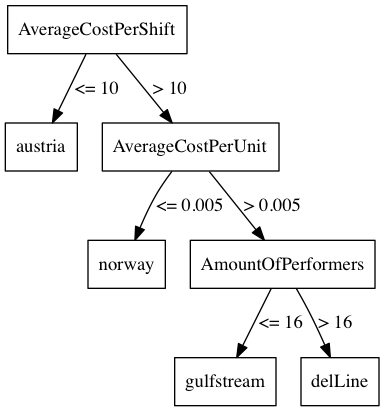
\includegraphics[scale=0.70]{tree1}
\end{figure}

Как видно из рисунка~\ref{tree1} , ключевыми признаками являются:
\begin{itemize}
\item $AverageCostPerShift$ / Средняя цена за использование смены исполнителем или транспортом 
\item $AverageCostPerUnit$ / Средняя цена за минуту (для исполнителя), метр (для транспорта)
\item $AmountOfPerformers$ / Количество исполнителей заказов
\end{itemize}

\subsection{Убираются три признака при построении классификатора}

Очень важно иногда убирать признаки, при тестировании, чтобы посмотреть, как поведет себя $F_1$ мера.
Некоторые признаки могут отрицательно влиять на классификацию.
На самом деле, отрицательно --- не значит плохо.
Просто если какой-то признак будет постоянно являться ключевым при определении принадлежности к тому или иному датасету, то это не совсем хорошо, поскольку важно собрать, как можно больше  различных признаков, которые будут являться ключевыми при классификации.
Например, в предыдущем пункте указаны признаки, по которым, если внедрить какие-нибудь данные из реальной жизни, классификатор не будет к этому готов.
Имеет место переобучение.

Далее мы <<зашумим>> три признака, которые влияли на результат в прошлой подглаве.

\begin{table}[!h]
	\centering
	\caption{Не используется признаки количества водителей, средняя цена за использование смены исполнителем или транспортом, средняя цена за минуту (для исполнителя), метр (для транспорта) }\label{tab2}
			\begin{tabu}{|*{18}{c|}}\hline
			                           &  1  & 2 & 3 & 4 & 5 & Среднее \\\hline
			Дерево Решений & 1.000 & 0.949 & 1.000  & 0.949 & 0.949 & 0.969 \\\hline
			SVM                    &  1.000 & 0.949 & 1.000  & 0.949 & 0.949 & 0.969 \\\hline
			LogReg              & 0.949 & 0.949 & 1.000  & 0.949 & 0.899 & 0.949  \\\hline
			RandomForest &1.000 & 0.949 & 1.000 &  0,949  & 0.949 & 0.969 \\\hline
		\end{tabu}
\end{table}

В целом, опираясь на таблицу~\ref{tab2}, можно сказать,что все типы показали отличный результат.
Чуть хуже повела себя логистическая регрессия.

\begin{figure}[h]
	\caption{<<Дерево решений>> в случае с 3 зашумленными признаками \label{tree2}} \centering
	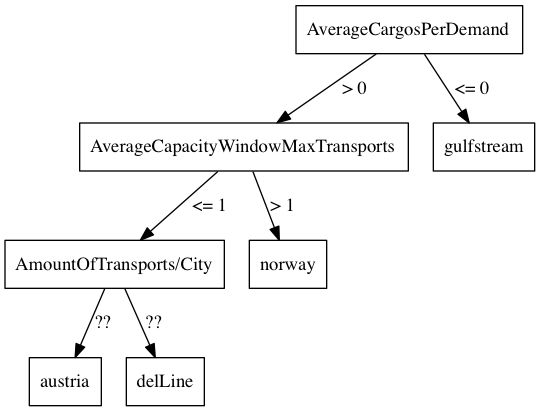
\includegraphics[scale=0.70]{tree2}
\end{figure}

Как видно из рисунка~\ref{tree2} , ключевыми признаками являются:

\begin{itemize}
	\item $AverageCargosPerDemand $ / Среднее количество грузов в заказах
	\item $AverageCapacityWindowMaxTransports$ / Количество транспорта, который может работать в локации одновременно
\end{itemize}

Собственно $AverageCargosPerDemand $ действительно очень правильно определяет класс \textit{gulfstream}, так он очень существенно выделяется количеством грузов в заказах.
$AverageCapacityWindowMaxTransports$ чаще всего пишется тестировщиками, так что по этому признаку очень тяжело судить, его можно отбросить.

\subsection{<<Зашумляется>> еще один признак при построении классификатора}

Далее исследование продолжается без четырех признаков, рассматриваемых выше.

\begin{table}[!h]
	\centering
	\caption{Не используются 4 признака, указанных выше в подглавах $3.3.1$ и $3.3.2$}\label{tab3}
	\begin{tabu}{|*{18}{c|}}\hline
	                          &  1  & 2 & 3 & 4 & 5 & Среднее \\\hline
	Дерево Решений & 1.000 & 0.949 & 1.000  & 1.000 & 0.949 & 0.980 \\\hline
	SVM                    &  1.000 & 0.949 & 1.000  & 1.000 & 0.949 & 0.980 \\\hline
	LogReg              & 0.949 & 0.949 & 1.000  & 1.000 & 0.949 & 0.969  \\\hline
	RandomForest &    0.949 & 0.949 & 0.949 &  0.949  & 0.899 & 0.940 \\\hline
\end{tabu}
\end{table}

Опираясь на таблицу~\ref{tab3}, можно заметить,что результаты на всех типа показаны одинаково неплохие.

\begin{figure}[h]
	\caption{Первый из встречающихся вариантов <<Дерева решений>> в случае с 4 <<зашумленными>> признаками \label{tree3}} \centering
	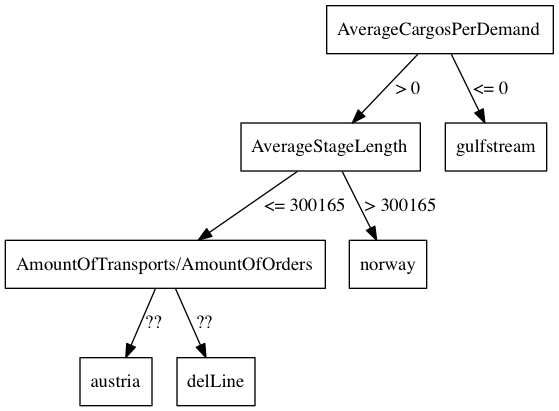
\includegraphics[scale=0.70]{tree3}
\end{figure}

\begin{figure}[h]
	\caption{Второй из встречающихся вариантов <<Дерева решений>> в случае с 4 <<зашумленными>> признаками \label{tree4}} \centering
	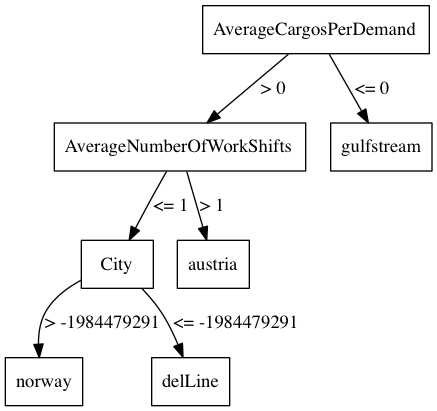
\includegraphics[scale=0.70]{tree4}
\end{figure}

Как видно из рисунка~\ref{tree3} и рисунка~\ref{tree4} , ключевыми признаками в данном случае чаще всего являлись:
\begin{itemize}
	\item $AverageStageLength$ / Средняя длительность временного отрезка в минутах (для исполнителя), длительность пути в метрах (для транспорта)
	\item $AverageNumberOfWorkShifts$ / Среднее количество рабочих смен для исполнителей
	\item $AmountOfOrders$ / Количество заказов
	\item $AmountOfTransports$ / Количество транспортых средств, выполняющих заказы
	\item $City$ / Город, где проводится доставка
\end{itemize}

Первый признак действительно грамотный для определения класса \textit{norway}, второй хорошо идентифицирует класс \textit{austria}.

Про последние 3 признака и их не слишком большую информативность, речь пойдет в следующем разделе.

\subsection{Дополнительные прогоны}

Признаки $AmountOfOrders$, $AmountOfTransports$, $City$ на тех данных, на которых происходит исследование, могут давать не всегда информативные результаты.Во многом, это связано со спецификой семплирования. К тому же город тоже очень сильно может перетягивать одеяло на себя по той причине, что данных очень мало, и регионы в датасетах практически все различные.

Попробуем посмотреть,что получится, если <<зашумить>> все неинформативные признаки, и те, что указаны в этом разделе.

\begin{table}[!h]
	\centering
	\caption{Дополнительные прогоны с <<зашумлением>> неинформативных признаков }
	\label{tab4}
			\begin{tabu}{|*{18}{c|}}\hline
			&  1  & 2 & 3 & 4 & 5 & Среднее \\\hline
			Дерево Решений & 1.000 & 0.949 & 0.949  & 1.000 & 1.000 & 0.980 \\\hline
			SVM                    &  0,949  & 0,949  & 0.949  & 1.000 & 0.949 & 0.960 \\\hline
			LogReg              & 0.675 & 0.764 & 0.804  & 0.709 & 0.719 & 0.734  \\\hline
			RandomForest    &   0,899  & 0,896 & 0.899 &  1.000 & 0.949 & 0.929 \\\hline
		\end{tabu}
\end{table}

Можно обратить внимание, на то, что на этих прогонах сильно <<просела>> LogReg, как и Random Forest.
Лучший результат показало <<Дерево Решений>>.

 Признаки чаще всего определялись из того множества, что было указано в предыдущих разделах.
 Без многих неинформативных признаков ключевыми также стали features, посчитанные по матрицам совместимости.
 Пример <<точного>> решения представлен на рисунке~\ref{tree5}.
 Здесь $F_1$ мера постоянно равнялась 1, на нижнем уровне менялись признаки, но они всегда относились к категории <<матрицы совместимости>>.

\begin{figure}[h]
	\caption{Пример <<Дерева Решений>>, в котором присутствуют признаки <<матрицы совместимости>> \label{tree5}} \centering
	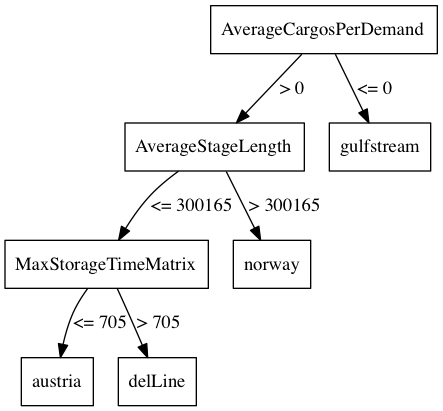
\includegraphics[scale=0.68]{tree5}
\end{figure}


\chapterconclusion

В данной главе речь идет об анализе данных, рассматривается практическая сторона решения.
Рассказывается про классы наборов данных, которые были рассмотрены.
Высчитывается метрика на нескольких моделях, выделяются ключевые признаки, делаются выводы.
Как можно заметить, лучший результат в среднем показывается при <<Дереве Решений>>.
Усредненная $F_1$ мера составляет 0.967.


%% Макрос для заключения. Совместим со старым стилевиком.
\startconclusionpage

В данной работе была рассмотрена важная и интересная бизнес-задача, необходимая компании VeeRoute.
С ее помощью компания сможет классифицировать новые наборы данных,на основании информации об известных.
На данные, которые уже есть у компании, имеется готовый набор конфигурационных файлов, который учитывает специфику бизнес-процессов и формат входного файла.
Указав машинным обучением в данной работой на то, к какой категории относится датасет, и по каким признакам это определяется, компания VeeRoute сможет уйти от ручной проверки, которая занимает очень много времени при большом количестве данных.
В данный момент, датасетов, к сожалению, не так много, поэтому достоверно оценить качество проведенного исследования достаточно проблематично. Но на данном этапе результаты, полученные в данной работе вполне удовлетворяют запросам компании.
Достигнута основная задача --- можно давать программе тестовую выборку датасетов, и она определит к катой категории из обучающей выборки принадлежит искомые объекты.



\printmainbibliography


\appendix

\chapter{Признаки для построения классификатора}

Ниже представлено название/описание, использованных для построения классификатора признаков.

\begin{itemize}
	\item AmountOfOrders / Количество заказов
	\item AmountOfPerformers / Количество исполнителей заказов
	\item AmountOfTransports / Количество транспортых средств, выполняющих заказы
	\item City / Город, где проводится доставка
	\item MaxStorageTimeMatrix / Матрица совместимости (состоит из максимального времени возможного нахождения груза заявки в данном отсеке)
	\item OnBoardMatrix / Матрица загрузки груза заявок, которые уже загружены в отсек транспорта
	\item OrderOrderMatrix / Матрица совместимости. Данная связь (OrderOrderRelations) используется для определения возможности перевозки грузов разных заказов в одном отсеке одного транспорта и одним исполнителем, данная совместимость интегральная, т.е. учитываются ограничения на все заявки (грузы) входящие в заказ
	\item PerformerOrderMatrix / Матрица совместимости. Данная связь (PerformerOrderRelations) используется для определения возможности исполнителя работать с определенным заказом (и всеми заявками, которые в него входят).
	\item PerformerTransportMatrix / Матрица совместимости. Данная связь (PerformerTransportRelations) используется для определения возможности исполнителя управлять определенным транспортным средством
	\item TransportLocationMatrix / Матрица совместимости. Данная связь (TransportLocationRelations) используется для определения возможности транспорта производить работу на конкретных локациях
	\item TransportType / Типы транспортов и количество, которые участвуют в маршрутизации
	\item AverageDistanceInLengthMatrix / Базовая матрица расстояний между точками, в метрах. Среднее расстояние между соседними точками
	\item RangTimeMatrix / Базовая матрица времен, необходимых на перемещения из каждой точки в каждую, в минутах. Ранг
	\item AverageTimeInTimeMatrix / Базовая матрица времен, необходимых на перемещения из каждой точки в каждую, в минутах. Среднее время перемещения между соседними точками.
	\item RangLengthMatrix / Базовая матрица расстояний между точками, в метрах. Среднее расстояние между соседними точками.
	\item AverageCostPerUnit / Средняя цена за минуту (для исполнителя), метр (для транспорта)
	\item AverageStageLength / Средняя длительность временного отрезка в минутах (для исполнителя), длительность пути в метрах (для транспорта)
	\item AverageCostPerShift / Средняя цена за использование смены исполнителем или транспортом
	\item AverageArrivalDuration / Среднее время на подъезд к локации
	\item AverageDepartureDuration / Среднее время на отъезд с локации
	\item AmountOfLocations / Количество локаций
	\item AverageCapacityTimeWindowDuration / Окна загрузки или разгрузки (CapacityWindow) для локаций определяют количество груза, которое локация способна отдать \ принять. Продолжительность среднего временное окно по всем локациям
	\item AverageCapacityWindowMaxTransports / Количество транспорта, который может работать в локации одновременно. Среднее количество такого транспорта по всем локациям,где есть окна загрузки или разгрузки
	\item CapacityWindowTypePICKUP / Количество окон на загрузку (перемещение груза из локации в транспорт)
	\item CapacityWindowTypeDROP / Количество окон на разгрузку (перемещение груза из транспорта в локацию)
	\item CapacityWindowTypeWORK / Количество окон на доступное время, когда возможна работа на локации
	\item AverageCargosCapacity / Средняя вместимость грузов по заказам
	\item AverageCargosPerDemand / Среднее количество грузов в заказах
	\item AverageEventDuration / Среднее время выполнения события, в минутах
	\item AverageHardTimeWindowDuration / Среднее жесткое временное окно для события. Продолжительность
	\item AverageEventSoftTimeWindowDuration / Среднее мягкое(желаемое) временное окно для события. Продолжительность
	\item AverageNumberOfPossibleEvents / Среднее количество событий в каждой заявке, выполнение любого из которых (из событий) дает выполнение заказа
	\item AverageCapacityTimeWindowFrom / Окна загрузки или разгрузки (CapacityWindow) для локаций определяют количество груза, которое локация способна отдать(принять). Cреднее начало временного окна по всем локациям
	\item AverageCapacityTimeWindowTo,1351.0,Окна загрузки или разгрузки (CapacityWindow) для локаций определяют количество груза, которое локация способна отдать (принять). Среднее окончание временного окна по всем локациям
	\item AverageEventHardTimeWindowFrom / Среднее жесткое временное окно для события. Конец окна
	\item AverageEventHardTimeWindowTo / Среднее жесткое временное окно для события. Начало окна
	\item AverageEventSoftTimeWindowFrom / Среднее мягкое (желаемое) временное окно для события. Начало окна
	\item AverageEventSoftTimeWindowTo / Среднее мягкое (желаемое) временное окно для события.Конец окна
	\item AverageStartBreakTime / Среднее время начала перерыва (использование данного параметра зависит от типа перерыва), в минутах
	\item AverageNumberOfBreaks / Среднее количество перерывов, в которое исполнители не доступны для выполнения заказов
	\item AverageDurationBreakTime / Средняя длительность перерыва, в минутах
	\item NumberOfBreakTypeBTFIXED / Количество перерывов, которые начинаются в указанное время (break time)
    \item NumberOfBreakTypeBTITERATIVE / Количество перерывов, которые необходимо выполнять раз в указанное количество минут (break time), при этом считается время работы driving time + waiting time.
    \item AverageNumberOfWorkShifts / Среднее количество рабочих смен для исполнителей
    \item AveragePerformerTimeWindowDuration / Среднее временное окно действия смены, в минутах. Продолжительность окна
    \item AveragePerformerTimeWindowFrom / Среднее временное окно действия смены, в минутах. Начало окна
    \item AveragePerformerTimeWindowTo / Среднее временное окно действия смены, в минутах. Конец окна
    \item AverageNumberOfBoxes / Среднее число отсеков ~--- часть транспорта, способная вмещать груз
    \item AverageNumberOfCapacitiesInBoxes / Среднее число вариантов вместимости в отсеках
    \item AverageBoxesCapacity / Средняя вместимость отсеков
    \item AverageTransportTimeWindowDuration / Среднее временное окно действия смены, в минутах. Продолжительность окна
    \item AverageTransportTimeWindowFrom / Среднее временное окно действия смены, в минутах. Начало окна
    \item AverageTransportTimeWindowTo / Среднее временное окно действия смены, в минутах. Начало окна	
\end{itemize}


\end{document}
